%\VignetteIndexEntry{contextual: Simulating Contextual Multi-Armed Bandit Problems in R (article)}
%\VignetteEngine{knitr::knitr}
%\VignetteKeyword{archivsit}
%\VignetteKeyword{package}
%\VignetteKeyword{vignette}
%\VignetteKeyword{LaTeX}
\documentclass[nojss]{jss}\usepackage[]{graphicx}\usepackage[]{color}
%% maxwidth is the original width if it is less than linewidth
%% otherwise use linewidth (to make sure the graphics do not exceed the margin)
\makeatletter
\def\maxwidth{ %
  \ifdim\Gin@nat@width>\linewidth
    \linewidth
  \else
    \Gin@nat@width
  \fi
}
\makeatother

\definecolor{fgcolor}{rgb}{0.345, 0.345, 0.345}
\newcommand{\hlnum}[1]{\textcolor[rgb]{0.686,0.059,0.569}{#1}}%
\newcommand{\hlstr}[1]{\textcolor[rgb]{0.192,0.494,0.8}{#1}}%
\newcommand{\hlcom}[1]{\textcolor[rgb]{0.678,0.584,0.686}{\textit{#1}}}%
\newcommand{\hlopt}[1]{\textcolor[rgb]{0,0,0}{#1}}%
\newcommand{\hlstd}[1]{\textcolor[rgb]{0.345,0.345,0.345}{#1}}%
\newcommand{\hlkwa}[1]{\textcolor[rgb]{0.161,0.373,0.58}{\textbf{#1}}}%
\newcommand{\hlkwb}[1]{\textcolor[rgb]{0.69,0.353,0.396}{#1}}%
\newcommand{\hlkwc}[1]{\textcolor[rgb]{0.333,0.667,0.333}{#1}}%
\newcommand{\hlkwd}[1]{\textcolor[rgb]{0.737,0.353,0.396}{\textbf{#1}}}%
\let\hlipl\hlkwb

\usepackage{framed}
\makeatletter
\newenvironment{kframe}{%
 \def\at@end@of@kframe{}%
 \ifinner\ifhmode%
  \def\at@end@of@kframe{\end{minipage}}%
  \begin{minipage}{\columnwidth}%
 \fi\fi%
 \def\FrameCommand##1{\hskip\@totalleftmargin \hskip-\fboxsep
 \colorbox{shadecolor}{##1}\hskip-\fboxsep
     % There is no \\@totalrightmargin, so:
     \hskip-\linewidth \hskip-\@totalleftmargin \hskip\columnwidth}%
 \MakeFramed {\advance\hsize-\width
   \@totalleftmargin\z@ \linewidth\hsize
   \@setminipage}}%
 {\par\unskip\endMakeFramed%
 \at@end@of@kframe}
\makeatother

\definecolor{shadecolor}{rgb}{.97, .97, .97}
\definecolor{messagecolor}{rgb}{0, 0, 0}
\definecolor{warningcolor}{rgb}{1, 0, 1}
\definecolor{errorcolor}{rgb}{1, 0, 0}
\newenvironment{knitrout}{}{} % an empty environment to be redefined in TeX

\usepackage{alltt}

\usepackage[utf8]{inputenc}
\usepackage{color}

%% packages added by RvE
\usepackage{amssymb}
\usepackage{amsmath}
\usepackage{txfonts}
\usepackage{mathdots}
\usepackage{float}
%\usepackage[classicReIm]{kpfonts}
%\usepackage[pdftex]{graphicx}

\usepackage{natbib}
\usepackage[british]{babel} % for correct word hyphenation
\raggedbottom % for blank spaces at the bottom (e.g., references section)
%\setcounter{tocdepth}{3} % for table of contents
%\setcounter{secnumdepth}{3} % setting level of numbering
%%%%%%%%%%%%%%%%%%%%%%%%%%%%%%
%% declarations for jss.cls %%%%%%%%%%%%%%%%%%%%%%%%%%%%%%%%%%%%%%%%%%
%%%%%%%%%%%%%%%%%%%%%%%%%%%%%%

%% almost as usual
\author{Robin van Emden\\JADS \And
  Eric Postma\\Tilburg University \And
  Maurits Kaptein\\Tilburg University}

\title{\pkg{contextual}: Simulating Contextual Multi-Armed Bandit Problems in R}

%% for pretty printing and a nice hypersummary also set:
\Plainauthor{Robin van Emden, Eric Postma, Maurits Kaptein} %% comma-separated
\Plaintitle{contextual: Simulating Contextual Multi-Armed Bandit Problems in R} %% without formatting
\Shorttitle{\pkg{contextual}} %% a short title (if necessary)

%% an abstract and keywords
\Abstract{
The elegance with which many statistical and reinforcement problems can be framed as (contextual) Multi-Armed Bandit problems, together with a proliferation of powerful Bandit algorithms and a growing body of analytically oriented research has led Multi-Armed Bandit methods to be applied to ever more real-world partial information sequential decision problems, from online advertising and recommender systems to the optimization of clinical trials and personalized medicine. At the same time, tools to comprehensively compare Bandit algorithms on simulated and real-life offline data seem to be lagging behind. To help close this gap between analytical research and real life application, this paper introduces the R package \pkg{contextual}, a user friendly and easily extensible framework that facilitates the comparison of, amongst others, contextual an non-contextual Bandit policies through both simulation and offline analysis. }

\Keywords{contextual multi-armed bandits, simulation, sequential experimentation, \proglang{R}}
\Plainkeywords{contextual multi-armed bandits, simulation, sequential experimentation, R}

%% at least one keyword must be supplied

%% publication information
%% NOTE: Typically, this can be left commented and will be filled out by the technical editor
%% \Volume{50}
%% \Issue{9}
%% \Month{June}
%% \Year{2012}
%% \Submitdate{2012-06-04}
%% \Acceptdate{2012-06-04}

%% The address of (at least) one author should be given
%% in the following format:
\Address{
  Robin van Emden\\
  Jheronimus Academy of Data Science\\
  Den Bosch, the Netherlands\\
  E-mail: \email{robin@pwy.nl} \\
  URL: \url{pavlov.tech}\\
  \linebreak
  Eric O. Postma\\
  Tilburg University\\
  Communication and Information Sciences\\
  Tilburg, the Netherlands\\
  E-mail: \email{e.o.postma@tilburguniversity.edu}\\
  \linebreak
  Maurits C. Kaptein\\
  Tilburg University\\
  Statistics and Research Methods\\
  Tilburg, the Netherlands\\
  E-mail: \email{m.c.kaptein@uvt.nl}\\
  URL: \url{www.mauritskaptein.com}\\
}

%% It is also possible to add a telephone and fax number
%% before the e-mail in the following format:
%% Telephone: +43/512/507-7103
%% Fax: +43/512/507-2851

%% for those who use Sweave please include the following line (with % symbols):
%% need no \usepackage{Sweave.sty}

%% end of declarations %%%%%%%%%%%%%%%%%%%%%%%%%%%%%%%%%%%%%%%%%%%%%%%
\IfFileExists{upquote.sty}{\usepackage{upquote}}{}
\begin{document}

A vignette for the \cite{contextual} paper.

%% include your article here, just as usual
%% Note that you should use the \pkg{}, \proglang{} and \code{} commands.







\section{Introduction}
%% Note: If there is markup in \(sub)section, then it has to be escape as above.

In a Multi-Armed Bandit (MAB) problem, an agent follows the advice of an algorithm or \textquotedblleft{}policy\textquotedblright{} in order to optimize the overall reward it receives in a sequential decision problem with limited information. That is, a MAB policy advices an agent when to explore new options and when to exploit known ones \textendash{} where, importantly, for each decision, at each time step t, the only new information the agent acquires is the reward for its latest decision. The agent remains in the dark about the potential rewards of the unchosen options and about any other information outside of current and past rewards and choices made.

In that respect, MAB problems reflect dilemmas we all encounter on a daily basis: do you stick to what you know and receive an expected result ("exploit") or choose something you don't know all that much about and potentially learn something new ("explore")?

\begin{itemize}
\item Do you feed your next coin to the one-armed bandit that paid out last time, or do you test your luck on another arm, on another machine?
\item When going out to dinner, do you explore new restaurants, or do you exploit familiar ones?
\item Do you stick to your current job, or explore and hunt around?
\item Do I keep my current stocks, or change my portfolio and pick some new ones?
\item As an online marketer, do you try a new ad, or keep the current one?
\item As a doctor, do you treat your patients with tried and tested medication, or do you prescribe a new and promising experimental treatment?
\end{itemize}

Though MAB models are already powerful of their own accord, a recent generalization, known as the \pkg{contextual} Multi-Armed Bandit (cMAB), adds one important element to the equation: in addition to past decisions and their rewards, cMAB agents are able to make use of side information on the state of the world at each t, right before making their decision. In other words, an agentthat follows the advice of a cMAB policy may decide differently in different contexts.

This access to side information has proven to make cMAB algorithms an even better fit to many real-life decision problems. Do you show a certain add to returning customers, to new ones, or both? Do you prescribe a different treatment to male patients, female patients, or both? In the real world, it appears almost no choice exists without its context. So it may be no surprise that cMAB algorithms have found many uses: from recommender systems and advertising to health apps and personalized medicine. This practical applicability has led to a multitude of policies, each with their own strengths and weaknesses.

Still, though cMAB algorithms have gained much traction in both research and industry, they have mostly been studied mathematically and analytically \textendash{} comparisons on simulated, and, importantly, real-life large-scale offline \textquotedblleft{}partial label\textquotedblright{} data sets have been lacking. To this end, the current paper introduces the \pkg{contextual} R package. A package that aims to facilitate the simulation, offline comparison, and evaluation of (Contextual) Multi-Armed bandit policies. Though there exists one R package for basic MAB analysis, there is, as of yet, no extensible and widely applicable R package that is able to analyze and compare, respectively, basic K-armed, Continuum, Adversarial and Contextual Multi-Armed Bandit Algorithms on either simulated or online data.

In section 2, this paper will continue with a more formal definition of MAB and a CMAB problems. In section 3, we will continue with an overview of \pkg{contextual}’s general implementation. In section 4, we list our implemented polices, and simulate a MAB and a cMAB policy. In section 5, we demonstrate how easy it is to add and simulate your own custom policy. In section 6, we replicate two papers, thereby demonstrating how to test policies on offline data sets. Finally, in section  7, we will go over some of the additional features in the package, and conclude with some comments on the current state of the package and possible enhancements.

\section{Contextual Multi-Armed Bandits}
%% Note: If there is markup in \(sub)section, then it has to be escape as above.

On formalizing our Multi-Armed Bandit problem, the aforementioned sequential decision maker's exploit/explore dilemma can be captured by defining a finite set (or \textbf{bandit)} of \textit{K} i.i.d. options (the \textbf{arms }of the bandit\textbf{) }each with their own, unknown\textbf{, }reward distribution \textit{v${}_{1}$,{\dots},v${}_{k}$} with means \textit{$\mu$ {\dots} $\mu$${}_{k}$}. Next we define an \textbf{agent}, who has to decide between the exploration of unknown arms and the exploitation of known arms in \textit{K} in order to maximize its total\textbf{ reward} (that is, to maximize its cumulative reward $\sum_{t=1}^T r_t$ \footnote{or to minimize its cumulative or expected regret}) over a period of time $T$ by following the advice of a \textbf{policy $\boldsymbol{\piup}$} which keeps track of \textbf{parameters} \textbf{\textit{$\boldsymbol{\theta}$}}\textit{ }that are updated when new information (reward \textit{r} awarded by the bandit when the agent has chosen an arm) becomes available. This process is repeated \textit{T} times, where \textit{T} is often defined as the Bandit's "horizon".

That is, an agent repeats the following lines one at a time at each time step \textit{t }in \textit{t}=1,2,{\dots},\textit{T}:

\begin{enumerate}
         \item[1a)] Agent asks policy $\piup$ which of the bandit's K arms to choose
         \item[1b)] Policy $\piup$ advices action \textit{a${}_{t}$} based on the state of a set of parameters \textit{$\theta$${}_{t}$}
         \item[2a)] Agent does action \textit{a${}_{t}$} by playing the suggested bandit arm.
         \item[2b)] Bandit rewards the agent with reward \textit{r${}_{t}$ }for action \textit{a${}_{t}$},
         \item[3a)] Agent sends the reward\textit{ r${}_{t}$ }to policy $\piup$
         \item[3b)] Policy $\piup$ uses \textit{r${}_{t}$} to update the policy's set of parameters\textit{ $\theta$${}_{t}$}
\end{enumerate}


\begin{figure}[H]
  \centering
    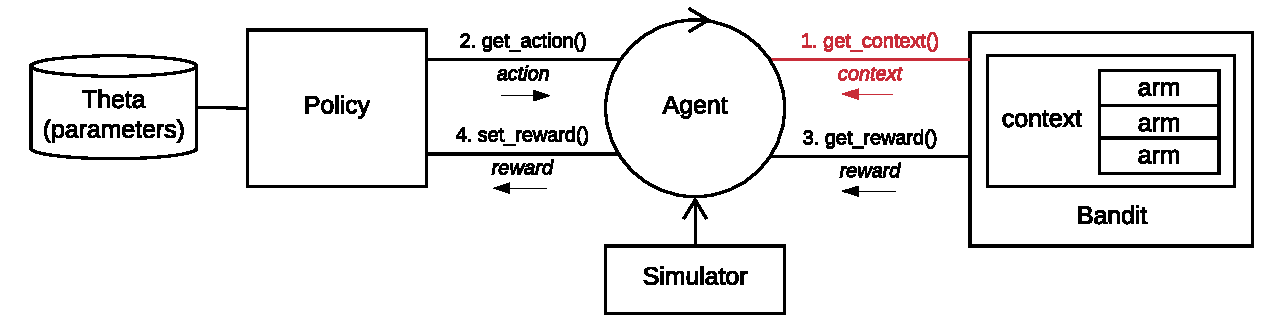
\includegraphics[width=.99\textwidth]{fig/cmab_chart}
    \label{fig:mab_chart}
      \caption{Overview MAB formalization towards \pkg{contextual}'s implementation}
\end{figure}

To allow for side information, that is, to generalize this formalization to a \textit{contextual} Multi-Armed Bandit model, the model needs just one additional step. Again, an agent repeats the following lines for each time step \textit{t} in \textit{t}=1,2,{\dots},\textit{T}:

\begin{enumerate}
         \item[1a)] Agent checks the bandit for side information that might influence the expression of its arms
         \item[1b)] Bandit returns feature vector \textit{Xt }
         \item[2a)] Agent asks policy $\piup$ which of the bandit's K arms to choose given \textit{Xt}
         \item[2b)] Given \textit{Xt}, policy $\piup$ advices action \textit{a${}_{t}$} based on the state of a set of parameters \textit{$\theta$${}_{t}$${}_{  }$}
         \item[3a)] Agent does action \textit{a${}_{t}$} by playing the suggested bandit arm.
         \item[3b)] Bandit rewards the agent with reward \textit{r${}_{t}$ }for action \textit{a${}_{t}$},
         \item[4a)] The agent sends the reward\textit{ r${}_{t}$ }to policy $\piup$
         \item[4b)] Policy $\piup$ uses \textit{r${}_{t}$} to update the policy's set of parameters\textit{ $\theta$${}_{t}$${}_{  }$}given \textit{Xt}
\end{enumerate}

\begin{figure}[H]
  \centering
    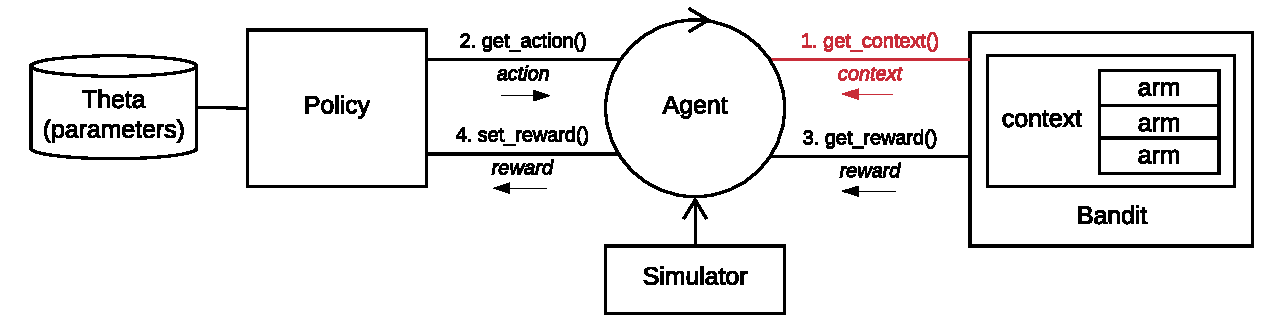
\includegraphics[width=.99\textwidth]{fig/cmab_chart}
    \label{fig:cmab_chart}
      \caption{Overview of cMAB formalization towards \pkg{contextual}'s implementation}
\end{figure}

As a matter of fact, by setting feature vector \textit{X} to [1] for each \textit{t} in step 1b, the suggested cMAB model perfectly emulates a non-contextual MAB model, easing the comparison and implementation of both MAB and cMAB substantially

\section{Implementation}
%% Note: If there is markup in \(sub)section, then it has to be escape as above.

In the canonical multi-armed bandit (MAB) problem a gambler faces a number of slot machines, each with a potentially different payoff. It is the gamblers goal to make as much profit (or, in the case of gambling, as little loss) as possible by sequentially choosing which machine to play, learning from the observations as she goes along.



\begin{knitrout}
\definecolor{shadecolor}{rgb}{0.969, 0.969, 0.969}\color{fgcolor}\begin{kframe}
\begin{alltt}
\hlkwd{library}\hlstd{(}\hlstr{"contextual"}\hlstd{)}

\hlstd{bandit}      \hlkwb{<-} \hlstd{BasicBandit}\hlopt{$}\hlkwd{new}\hlstd{()}

\hlstd{bandit}\hlopt{$}\hlkwd{set_weights}\hlstd{(}\hlkwd{c}\hlstd{(}\hlnum{0.1}\hlstd{,} \hlnum{0.9}\hlstd{))}

\hlstd{policy}      \hlkwb{<-} \hlstd{EpsilonGreedyPolicy}\hlopt{$}\hlkwd{new}\hlstd{()}

\hlstd{agent}       \hlkwb{<-} \hlstd{Agent}\hlopt{$}\hlkwd{new}\hlstd{(policy, bandit)}

\hlstd{simulation}  \hlkwb{<-} \hlstd{Simulator}\hlopt{$}\hlkwd{new}\hlstd{(agent,}
                             \hlkwc{horizon} \hlstd{=} \hlnum{100L}\hlstd{,}
                             \hlkwc{simulations} \hlstd{=} \hlnum{100L}\hlstd{,}
                             \hlkwc{worker_max} \hlstd{=} \hlnum{1}\hlstd{)}

\hlstd{history}     \hlkwb{<-} \hlstd{simulation}\hlopt{$}\hlkwd{run}\hlstd{()}

\hlstd{Plot}\hlopt{$}\hlkwd{new}\hlstd{()}\hlopt{$}\hlkwd{grid}\hlstd{(history)}
\end{alltt}
\end{kframe}
\end{knitrout}

For results, see Figure \ref{fig:fig1} on page \pageref{fig:fig1}.


\begin{center}
\begin{knitrout}
\definecolor{shadecolor}{rgb}{0.969, 0.969, 0.969}\color{fgcolor}\begin{figure}
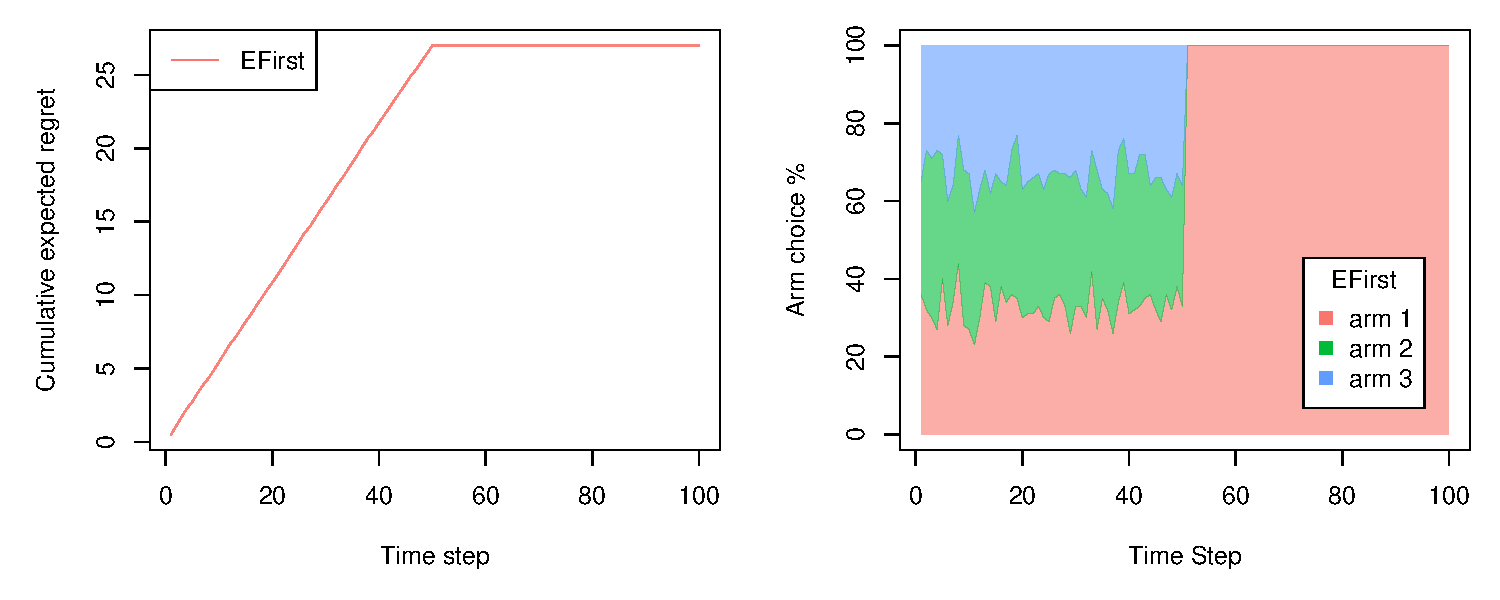
\includegraphics[width=\maxwidth]{fig/fig1-1} \caption[Epsilon Greedy]{Epsilon Greedy}\label{fig:fig1}
\end{figure}


\end{knitrout}
\end{center}

\section{Object orientation: extending contextual}
%% Note: If there is markup in \(sub)section, then it has to be escape as above.

The R6 package allows the creation of classes with reference semantics, similar to R's built-in reference classes. Compared to reference classes, R6 classes are simpler and lighter-weight, and they are not built on S4 classes so they do not require the methods package. These classes allow public and private members, and they support inheritance, even when the classes are defined in different packages.

One R6 class can inherit from another. In other words, you can have super- and sub-classes.

Subclasses can have additional methods, and they can also have methods that override the superclass methods. In this example of a custom \pkg{contextual} bandit, we’ll extend BasicBandit and override the initialize() method..

\section{Special features}
%% Note: If there is markup in \(sub)section, then it has to be escape as above.

For instance, quantifying variance..

\section{The art of optimal parallelisation}
%% Note: If there is markup in \(sub)section, then it has to be escape as above.

There is a very intersting trade of between the amount of parallelisation (how many cores, nodes used) the resources needed to compute a certain model, and the amount of data going to and fro the cores.

PERFORMANCE DATA  ------------------------------------------------------------

on 58  cores:    k3*d3 * 5 policies * 300  * 10000 --\textgreater{} 132 seconds

on 120 cores:    k3*d3 * 5 policies * 300  * 10000 --\textgreater{} 390 seconds

---

on 58  cores:    k3*d3 * 5 policies * 3000 * 10000 --\textgreater{} 930 seconds

on 120 cores:    k3*d3 * 5 policies * 3000 * 10000 --\textgreater{} 691 seconds



\section{Extra greedy UCB}
%% Note: If there is markup in \(sub)section, then it has to be escape as above.

In the canonical multi-armed bandit (MAB) problem a gambler faces a number of slot machines, each with a potentially different payoff. It is the gamblers goal to make as much profit (or, in the case of gambling, as little loss) as possible by sequentially choosing which machine to play, learning from the observations as she goes along.


\section{Conclusions}
\label{sec:conc4}

The goal of a data analysis is not only to answer a research question based on data but also to collect findings that support that answer. These findings usually take the form of a~table, plot or regression/classification model and are usually presented in articles or reports.

\section{Acknowledgments}

Thanks go to CCC.

%\bibliographystyle{apacite}
\bibliography{jss}

\end{document}
